\documentclass{article}

\usepackage[utf8]{inputenc}
\usepackage[T1]{fontenc}
\usepackage{amsmath}
\usepackage{amsfonts}
\usepackage{amssymb}
\usepackage[version=4]{mhchem}
\usepackage{stmaryrd}
\usepackage{bbold}
\usepackage{graphicx}
\usepackage{adjustbox}
\usepackage{tocloft}   % For TOC formatting
\usepackage{geometry}  % For margins
\usepackage{titlesec}  % For section formatting
\usepackage{fancyhdr}
\usepackage{float}
\usepackage[stable]{footmisc}
\usepackage{hyperref}  % For clickable links in TOC (load last)
\usepackage{mdframed}  
\usepackage{listings}  



% Document styling
\geometry{margin=1in}

% Customize section formatting (option 2: let titlesec handle the label)
\titleformat{\section}
  {\normalfont\Large\bfseries} % format
  {\thesection}                % label
  {0.5em}                      % separation
  {\rule{\textwidth}{0.4pt}\vspace{0.5em}\newline} % before-code

% adding a header
\pagestyle{fancy}
\fancyhf{}
\lhead{Problem Set 2}
\rhead{Henrik Berger - Romain Fernex}
\cfoot{ \thepage}
\renewcommand{\headrulewidth}{0.8pt}

\title{Problem Set 2 - Macroeconomics}
\author{Henrik Berger - Romain Fernex}
\date{February 2025}

\begin{document}

\maketitle
\tableofcontents
\newpage

\section{Literature review}

\begin{figure}[H]
    \centering
    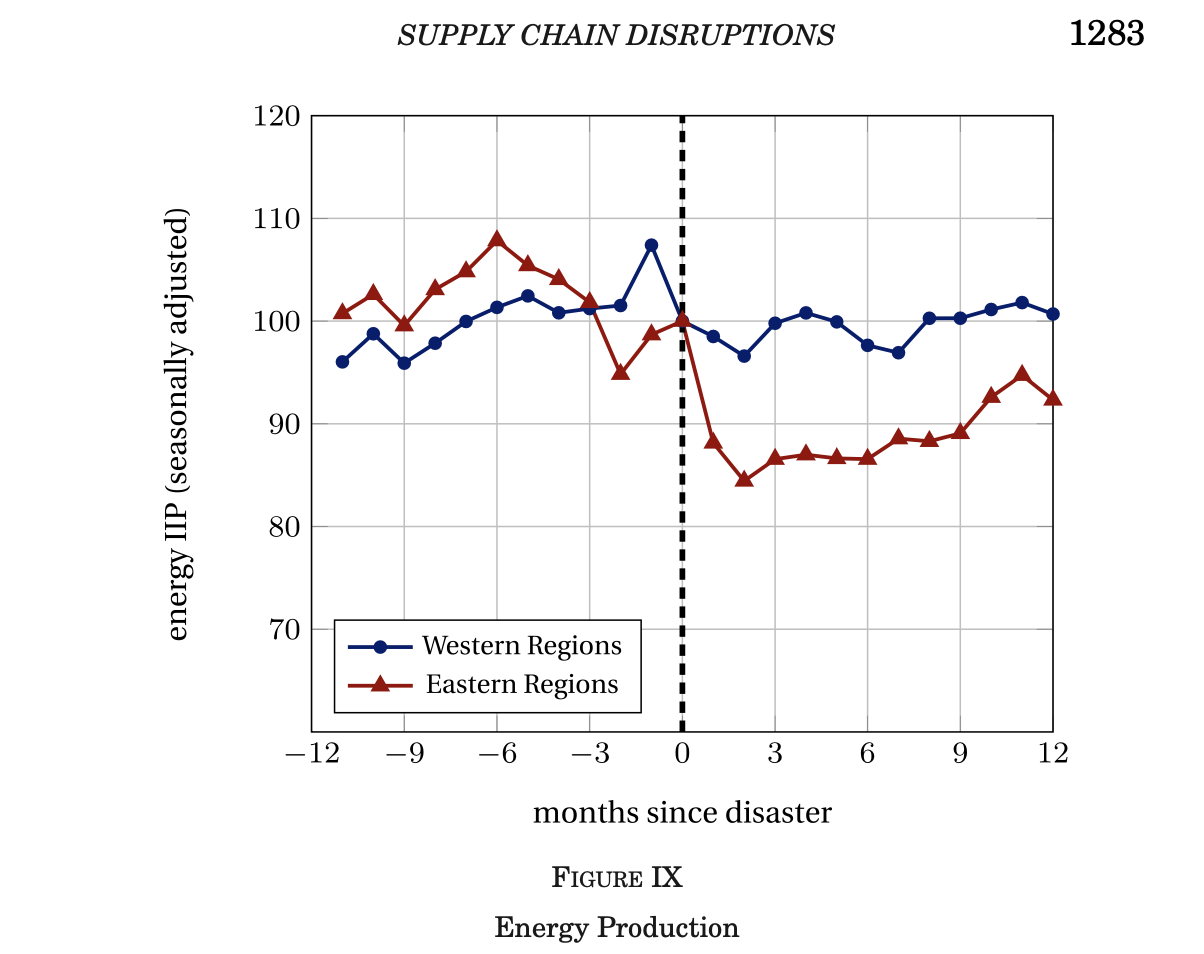
\includegraphics[width=0.8\textwidth]{figures/Screenshot 2025-10-02 at 9.56.48 PM.png}
    \caption{Impact of the 2011 Tohoku Earthquake on Japanese energy supply (breakdown East/West)}
    \label{fig: Impact of the 2011 Tohoku Earthquake on Japanese energy supply (breakdown East/West)}
\end{figure}
Figure IX shows the evolution of electricity production in eastern and western Japan around the time of the 2011 earthquake. The line for the east drops sharply after March 2011, reflecting the sudden loss of generating capacity, while the line for the west remains almost perfectly flat. This contrast is important because it rules out the idea that the whole country was hit by a single, uniform energy shortage. Instead, the shock was geographically concentrated, which makes it a genuinely idiosyncratic event. The authors use this fact to strengthen their broader argument. If the fall in output that they observe across many firms were simply due to a nationwide drop in electricity, then their results would not really tell us much about supply-chain transmission. But when they restrict the analysis to firms located in western Japan, which did not suffer power cuts, they still find the same patterns of downstream and upstream propagation. This means that the disruption spreads through firm-to-firm relationships rather than just through one big common shock. The figure therefore plays a crucial role in the paper: it visually separates localized infrastructure damage from the network effects the authors want to measure, and it illustrates how a shock that is small in geographical scope can ripple outward through production linkages.

\section{Exercise I}

\subsection{Part A}
\subsubsection{1)}
Lets denote $U = u(c_0)+E(u(c_1))  =u(c_0) + \frac{1}{2}u(c_1^G)+\frac{1}{2}u(c_1^B)$, with $u:c\xrightarrow{} ln(c)$.
The Coefficient of relative risk aversion (CRRA) is given by : $$CRRA(u) = -c\frac{u''(c)}{u'(c)}$$
Hence the following : 
$$CRRA (u) = -c\frac{\frac{-1}{c^2}}{\frac{1}{c}}=1$$

\subsubsection{2)}
Let's compute the aggregate income in the bad state of the economy : we denote $\omega$ the states of the world and $B$ the bad state 
$$\begin{aligned}y_1^B = E[y|\omega=B] = (1-\lambda)\mu+\lambda(1-\frac{\phi}{\lambda})\mu &= (1-\lambda)\mu + \lambda\mu - \phi \mu\\
&=(1-\phi )\mu
\end{aligned}$$
As expected, the aggregate income in this state of the world does not depend on the idiosyncratic risk induced by $\lambda$. 

\subsubsection{3)}
We need to consider two separate cases for the budget constraints : the complete market case and the incomplete market case\\
In the complete market case, the agent is only subject to aggregate risk so he faces the following constraints : 
$$\left\{\begin{aligned}
    &c_0 = \mu-p_2a_2-p_1a_1-qb\\
    &c_1^G= \mu +b-a_2+(1+\pi_1)a_1\\
    &c_1^B = (1-\phi)\mu + b -a_1+(1+\pi_2)a_2
\end{aligned}\right.$$
Now let's place ourselves in the incomplete market case : the agent now faces both aggregate and idiosyncratic risk as he cannot fully insure against the latter. Let's denote $c_1^{B,u}$ consumption in the bad state when the agent is not affected (still gets $\mu$) and $c_1^{B,a}$ when the agent is affected (gets $(1-\frac{\phi}{\lambda})\mu$).
$$\left\{\begin{aligned}
    &c_0 = \mu -p_2a_2-p_1a_1-qb\\
    &c_1^G = \mu + b-a_2+(1+\pi_1)a_1\\
    &c_1^{B,u} = \mu +b-a_1+(1+\pi_2)a_2\\
    &c_1^{B,a}= (1-\frac{\phi}{\lambda})\mu + b -a_1 + (1+\pi_2)a_2
\end{aligned}\right.$$

\subsection{Part B}
\subsubsection{1)}
The optimization program is the following : 
$$\begin{aligned}
    \max _{b,a_1,a_2} ln(c_0) + \frac{1}{2}ln(c_1^G)+\frac{1}{2}ln(c_1^B) \\
    \text{s.t }\left\{\begin{aligned}
    &c_0 = \mu-p_2a_2-p_1a_1-qb\\
    &c_1^G= \mu +b-a_2+(1+\pi_1)a_1\\
    &c_1^B = (1-\phi)\mu +  b-a_1+(1+\pi_2)a_2
\end{aligned}\right.
\end{aligned}$$
Substituting the constraints in the objective function, we can write : 
$$\max_{b,a_1,a_2} ln(\mu-p_2a_2-p_1a_1-qb) +  \frac{1}{2}ln(\mu +b-a_2+(1+\pi_1)a_1) + \frac{1}{2}ln((1-\phi)\mu +  b-a_1+(1+\pi_2)a_2)$$

\subsubsection{2)}
Let's derive the FOC's for the above optimization program : we denote $U$ the objective function
$$\begin{aligned}
    \frac{\partial U}{\partial b} &= 0 \Leftrightarrow \frac{-q}{c_0}+\frac{1}{2} (\frac{1}{c_1^G}+\frac{1}{c_1^B}) =0 \Leftrightarrow q = [\frac{1}{c_1^G}+\frac{1}{c_1^B}]\frac{c_0}{2}\\
     \frac{\partial U}{\partial a_1} &= 0 \Leftrightarrow \frac{-p_1}{c_0}+\frac{1}{2}(\frac{1+\pi_1}{c_1^G}-\frac{1}{c_1^B}) = 0 \Leftrightarrow p_1 = [\frac{1+\pi_1}{c_1^G}-\frac{1}{c_1^B}]\frac{c_0}{2}\\
     \frac{\partial U}{\partial a_2} &= 0 \Leftrightarrow \frac{-p_2}{c_0}-\frac{1}{2}(\frac{1}{c_1^G}-\frac{1+\pi_2}{c_1^B})=0\Leftrightarrow p_2 = [\frac{1+\pi_2}{c_1^B}-\frac{1}{c_1^G}]\frac{c_0}{2}
\end{aligned}$$
We assume that assets are priced considering exogenous consumption profile and equal to the income. Then, we replace $c_0,c_1^G$ and $c_1^B$ by their values to solve for asset prices in the complete market : 
$$\begin{aligned}
    q &= \frac{1}{2}[1+\frac{1}{1-\phi}]\\
    p_1 &= \frac{1}{2}[(1+\pi_1)-\frac{1}{1-\phi}]\\
    p_2 &= \frac{1}{2}[\frac{1+\pi_2}{1-\phi}-1]
\end{aligned}$$
Let's now write the ratio of $p_1$ and $p_2$ on $q$ : 
$$\begin{aligned}
    \frac{p_1}{q} &= \frac{(1+\pi_1)-\frac{1}{1-\phi}}{1+\frac{1}{1-\phi}}=\frac{\pi_1-\phi(1+\pi_1)}{2-\phi}\\
    \frac{p_2}{q} &= \frac{\frac{1+\pi_2}{1-\phi}-1}{1+\frac{1}{1-\phi}} =\frac{\pi_2+\phi}{2-\phi}
\end{aligned}$$
Firstly, we notice that both ratios do not depend on $\lambda$. This makes sense since, in the complete market setting, idiosyncratic risk does not come into play. Looking at comparative statics in $\phi$, we see that $\frac{p_2}{q}$ is increasing in $\phi$. Given that the payoff in the bad state depends negatively on $\phi$ and that $a_2$ provides utility in this state, the agent will be willing to pay more to get a greater payoff in the bad state when $\phi$ goes up. 
For the ratio involving $p_1$ the effect of $\phi$ appears to be ambiguous at first, let us compute its derivative to investigate whether one effect dominates : 
$$\frac{\partial \frac{p_1}{q}}{\partial \phi} = \frac{\pi_1-\phi(1+\pi_1)}{(2-\phi)^2}-\frac{1+\pi_1}{2-\phi} = \frac{-(2+\pi_1)}{(2-\phi)^2 }<0$$
Thus, $\frac{p_1}{q}$ decreases in $\phi$. This is in line with the fact that $a_1$ provides more utility in the good state and is thus more valuable when $\phi$ goes down (bad state is less punishing). 

\subsection{Part C}

\subsubsection{1)}
As we must know account for idiosyncratic risk, the optimization program is now the following : 
$$\begin{aligned}
    \max _{b,a_1,a_2} ln(c_0) + \frac{1}{2}ln(c_1^G)+\frac{1}{2}[\lambda ln(c_1^{B,a})+(1-\lambda)ln(c_1^{B,u})] \\
    \text{s.t }\left\{\begin{aligned}
    &c_0 = \mu -p_2a_2-p_1a_1-qb\\
    &c_1^G = \mu + b-a_2+(1+\pi_1)a_1\\
    &c_1^{B,u} = \mu +b-a_1+(1+\pi_2)a_2\\
    &c_1^{B,a}= (1-\phi)\mu + b -a_1 + (1+\pi_2)a_2
\end{aligned}\right.
\end{aligned}$$
As in part B, we substitute the constraints and get : 
$$\begin{aligned}
    \max _{b,a_1,a_2} &ln(\mu -p_2a_2-p_1a_1-qb) + \frac{1}{2}ln(\mu + b-a_2+(1+\pi_1)a_1)\\
    &+ \frac{1}{2}[\lambda ln((1-\phi)\mu + b -a_1 + (1+\pi_2)a_2) + (1-\lambda)ln(\mu +b-a_1+(1+\pi_2)a_2)]
\end{aligned} $$

\subsubsection{2)}
Let's compute the FOC's as we did in part B : 
$$\begin{aligned}
    \frac{\partial U}{\partial b} &= 0 \Leftrightarrow q= \frac{1}{2}[1+\frac{\lambda^2}{\lambda-\phi}+(1-\lambda)]\\
     \frac{\partial U}{\partial a_1} &= 0 \Leftrightarrow p_1 = \frac{1}{2}[\pi_1-\frac{\lambda^2}{\lambda -\phi}+\lambda]\\
     \frac{\partial U}{\partial a_2} &= 0 \Leftrightarrow p_2 = \frac{1}{2}[-1+(1+\pi_2)\{\frac{\lambda^2}{\lambda-\phi}+(1-\lambda)\}]
\end{aligned}$$
This gives us the following ratios: 
$$\begin{aligned}
    &\frac{p_1}{q} = \frac{\pi_1-\frac{\lambda^2}{\lambda-\phi}+\lambda}{1+\frac{\lambda^2}{\lambda-\phi}+(1-\lambda)} = \frac{\lambda(\pi_1-\phi)+\pi_1\phi}{\lambda (2+\phi)-2\phi}\\
    &\frac{p_2}{q} = \frac{-1+(1+\pi_2)\{\frac{\lambda^2}{\lambda-\phi}+(1-\lambda)\}}{1+\frac{\lambda^2}{\lambda-\phi}+(1-\lambda)} = \frac{\lambda\phi(1+\pi_2)+\pi_2(\lambda-1)}{2\lambda +\phi (\lambda -2)}
\end{aligned}$$
As the effect of $\lambda$ and $\phi$ is ambiguous for both ratios, we compute the derivatives and get :
$$\begin{aligned}
  &\frac{\partial\frac{p_1}{q}}{\partial \lambda }=  \frac{(\pi_1-\phi)(\lambda(2+\phi)-2\phi)-(2+\phi)(\lambda(\pi_1-\phi)+\pi_1\phi)}{(\lambda(2+\phi)-2\phi)^2} = \frac{-2\phi\pi_1+2\phi^2-2\phi\pi_1-\pi\phi^2}{(\lambda(2+\phi)-2\phi)^2} = \frac{-4\phi \pi_1+(2-\pi_1)\phi^2}{(\lambda(2+\phi)-2\phi)^2}\\
  &\frac{\partial\frac{p_1}{q}}{\partial \phi }= \frac{\lambda(2\pi_1-\lambda^2)}{(\lambda(2+\phi)-2\phi)^2}\\
   &\frac{\partial\frac{p_2}{q}}{\partial \lambda } = \frac{\pi_2[\pi_2(1-\frac{\phi}{2}-\phi^2)-\phi^2]}{(\lambda(2+\phi)-2\phi)^2}\\
   &\frac{\partial\frac{p_2}{q}}{\partial \phi } = \frac{\lambda^2(2+\pi_2)+3\lambda\pi_2-2\pi_2}{(\lambda(2+\phi)-2\phi)^2}
\end{aligned}$$

This result is foreseeable as homographic functions  are always monotone on each interval where they are defined. The sign of the derivative depends only on the numerator as the denominator is always positive, and the value of the numerator is independent of the variable of interest.
We cannot conclude decisively on how those ratios vary as a function of $\lambda$ and as a function of $\phi$ as the effect is ambiguous and depends on other parameters. 


\section{Exercise II}

\subsection{1)}
We have the following optimization program : 
$$\begin{aligned}\max_{a_{t+1},l_t}&\sum_{t=0}^{+\infty}\beta^tu(c_t-hc_{t-1},l_t) \text { with h<1}\\
&\text{s.t } c_t+a_{t+1}=(1+r_t)a_t+wl_t
\end{aligned}$$
Substituting the constraint in the objective function we get : 
$$\max_{a_{t+1},l_t}\sum_{t=0}^{+\infty} \beta^tu((1+r_t)a_t+wl_t-a_{t+1}-hc_{t-1},l_t)$$
Now, let's write down the Bellman equation of this problem with the value function : 
$$\begin{aligned}V(a,c_{-1}) &= u(\underbrace{(1+r)a+wl-a'-hc_{-1}}_{=c-hc_{-1}},l) + \beta V(a',\underbrace{(1+r)a+wl-a'}_{=c})
\end{aligned}\\
$$
\subsection{2)}
To solve for this let's get the Euler equation : 
\begin{itemize}
    \item We get the FOC's with respect to the control variables $a',l$ :
\begin{equation}\begin{aligned}
    &\text{(in $a'$)} \quad u_1(c-hc_{-1},l) = \beta V_1(a',c)-\beta V_2(a',c)\\
    &\text{(in $l$)} \quad wu_1(c-hc_{-1},l)+u_2(c-hc_{-1},l) = -w\beta V_2(a',c)
\end{aligned}\end{equation}
    \item We derive the envelope conditions using the state variables $a,c_{-1}$ \footnote{$l_{-1}$ could also be considered as a state variable however it does not enter directly the policy function so we omit it} : 
\begin{equation}\begin{aligned}
    &\text{(in $a$)} \quad V_1(a,c_{-1})=(1+r)u_1(c-hc_{-1},l)+\beta(1+r)V_2(a',c)\\
    &\text{(in $c_{-1}$)} \quad V_2(a,c_{-1}) = -hu_1(c-hc_{-1},l)
\end{aligned}\end{equation}
    \item We iterate (2) over $a,c_{-1},r,l$ : 
    \begin{equation}
        \begin{aligned}
            &V_1(a',c) = (1+r')u_1(c'-hc,l')+\beta (1+r')V_2(a'',c')\\
            &V_2(a',c) = -hu_1(c'-hc,l')
        \end{aligned}
    \end{equation}
    \item We combine (1) and (3) and get the following expression: 
    \begin{equation}
        \begin{aligned}
            u_1(c-hc_{-1},l) &= \beta [(1+r')u_1(c'-hc,l')+\beta (1+r')V_2(a'',c')]-\beta V_2(a',c) \\
            &= \beta[(1+r')u_1(c'-hc,l')+\beta(1+r')hu_1(c''-hc',l'')]+\beta hu_1(c'-hc,l') 
        \end{aligned}
    \end{equation}
    \item Hence, the EE is a follows:  
    $$EE : u_1(c-hc_{-1},l)-\beta hu_1(c'-hc,l') = \beta (1+r') [u_1(c'-hc,l')-\beta hu_1(c''-hc',l'')]$$
    \item similarly, we get the following equation for the work-leisure tradeoff : 
    $$W/L : u_2(c-hc_{-1},l) = w[\beta hu_1(c'-hc,l')-u_1(c-hc_{-1},l)]$$
\end{itemize}
Hence, the following pricing kernel : 
$$m' = \beta \frac{u_1(c'-hc,l')-\beta hu_1(c''-hc',l'')}{u_1(c-hc_{-1},l)-\beta hu_1(c'-hc,l')}\\= \frac{1}{1+r'}$$

\subsection{3)}
At the steady state, there are no variations across time so based on the EE we get : 
$$\begin{aligned}u_1(c-hc,l)(1-\beta h)=\beta(1+r)u_1(c-hc,l)(1-\beta h) &\Leftrightarrow 1  =\beta(1+r)\\
&\Leftrightarrow r =  \frac{1}{\beta}-1 
\end{aligned}
$$

\subsection{4)}
We wish to find the steady state optimal labor supply assuming that $a_t = 0$. To this end we can use the work-leisure tradeoff equation we obtained in (2), let's derive $u_1(c_t-hc_{t-1},l_t)$ and $u_2(c_t-hc_{t-1},l_t)$ : 
$$\begin{aligned}
    &u_1(c_t-hc_{t-1},l_t) = (c_t-hc_{t-1})^{-\sigma}\\
    &u_2(c_t-hc_{t-1},l_t) = -l_t^{\epsilon}
\end{aligned}$$
So we get the following equation for the work-leisure tradeoff : 
$$-l_t^{\epsilon} = w[\beta h (c_{t+1}-hc_t)^{-\sigma}-(c_t-hc_{t-1})^{-\sigma}]$$
Now we take the steady state so all time indexes disappear and we get :
$$\begin{aligned}
    &-l^\epsilon = w(\beta h-1)(c-hc)^{-\sigma}\\
    &\Leftrightarrow l^\epsilon = w(1-\beta h)(c-hc)^{-\sigma} \\
    &\Leftrightarrow l^\epsilon = w(1-\beta h)c^{-\sigma}(1-h)^{-\sigma}
\end{aligned}$$
Since $c=wl$ at the steady state based on the budget constraint with $a=0$, we get : 
$$\begin{aligned}
    &l^\epsilon = w(1-\beta h) w^{-\sigma}l^{-\sigma}(1-h)^{-\sigma}\\
    &\Leftrightarrow l^{\epsilon+\sigma} =(1-\beta h) w^{1-\sigma}(1-h)^{-\sigma}
\end{aligned}$$
the optimal labor denoted $l^*$ is thus as follows : 
$$l^* = [\frac{(1-\beta h)}{(1-h)^{\sigma}}w^{1-\sigma}]^{\frac{1}{\epsilon +\sigma }}$$
Let's derive this expression in h to get the variation of $l^*$ as a function of $h$ :  
$$\frac{dl^*}{dh}=\frac{l^*}{\epsilon+\sigma}(\frac{\sigma}{1-h}-\frac{\beta}{1-\beta h})$$
The response to a change in habit h is ambiguous as it depends on $\sigma$ and other parameters. 

\section{Exercise III}
Please find the associated notebook at the following link :  \href{https://pluto.land/n/mn6s26jq}{Notebook for Exercise 3} 

\section{Reference}
Vasco M Carvalho, Makoto Nirei, Yukiko U Saito, Alireza Tahbaz-Salehi, Supply Chain Disruptions: Evidence from the Great East Japan Earthquake, The Quarterly Journal of Economics, Volume 136, Issue 2, May 2021, Pages 1255–1321


\end{document}


